% =====================================================================
%  A economia-plataforma é fractal
%  Invariância de escala e especificidade composicional do vazamento
%  inter-regional — microrregiões do ES, UFs e o benchmark do porte.
%  Felipe Carvalho — PPGEco/UFES — Análise de Insumo-Produto (2026/1)
%
%  Números reproduzíveis de pesquisa/14_benchmark_ufs.py e
%  pesquisa/15_intra_es_fractal.py (saídas em outputs/). Convenção
%  spillover/feedback: Miller-Blair (inversa particionada).
% =====================================================================
\documentclass[11pt,a4paper]{article}
\usepackage[utf8]{inputenc}
\usepackage[T1]{fontenc}
\renewcommand{\abstractname}{Resumo}
\renewcommand{\refname}{Referências}
\usepackage{amsmath,amssymb}
\usepackage{booktabs}
\usepackage{graphicx}
\usepackage{geometry}
\usepackage{xcolor}
\usepackage{framed}
\usepackage[round,authoryear]{natbib}
\usepackage[hidelinks]{hyperref}
\geometry{margin=2.5cm}
\graphicspath{{../pesquisa/outputs/}{../figuras/}}
\definecolor{boxbg}{RGB}{246,243,234}\colorlet{shadecolor}{boxbg}

\title{\textbf{A economia-plataforma é fractal}\\[2pt]
\large Invariância de escala e especificidade composicional do vazamento
inter-regional \\ (microrregiões do Espírito Santo, 2015; unidades da
federação, 2008)}
\author{Felipe Carvalho\\
\small PPGEco --- UFES \quad$\cdot$\quad Análise de Insumo-Produto --- Prof. Dr. Celso Bissoli Sessa}
\date{julho de 2026}

\begin{document}
\maketitle
\thispagestyle{empty}

\begin{abstract}
\noindent
Trabalho anterior caracterizou o Espírito Santo (ES) como uma
\emph{economia-plataforma}: pequena, hiperaberta, com multiplicador que vaza de
forma concentrada para o núcleo São Paulo--Rio de Janeiro e \emph{feedback}
próximo de zero. Resta a objeção: esse padrão é \emph{específico} do ES ou
apenas a mecânica \emph{genérica} de qualquer região pequena e aberta? Este
artigo responde com dois testes complementares e uma virada de escala. Primeiro,
um \textbf{modelo nulo} sobre as 27 unidades da federação (2008) mostra que as
três métricas de insumo-produto da plataforma --- vazamento do multiplicador,
razão de \emph{feedback} e concentração do destino --- são, em grande parte,
\emph{função do porte}: a razão de \emph{feedback} cresce com o tamanho da
unidade ($R^2=0{,}59$), e o ES \emph{não} é \emph{outlier} em nenhuma delas
(escores-$z$ de $+0{,}45$, $-0{,}05$ e $+0{,}03$). Sua quase-nulidade de
\emph{feedback} é o que se espera para o seu porte. Segundo, aplicando o mesmo
aparato uma escala abaixo --- ao sistema inter-regional das \textbf{10
microrregiões} do ES (2015) ---, o padrão \emph{reproduz-se fractalmente}: a
Região Metropolitana (Grande Vitória) concentra 62\% da produção e retém o
multiplicador (vazamento de 8\%), enquanto a periferia primário-exportadora
vaza encadeamento \emph{para a metrópole} (até 76\% do \emph{spillover}); a
razão de \emph{feedback} volta a crescer com o porte, agora com $R^2=0{,}91$. A
extração hipotética da metrópole derruba em 13\% a produção das demais
microrregiões. A conclusão reposiciona a tese: a \emph{mecânica}-plataforma é
uma regularidade de \emph{posição e porte}, invariante de escala; o que
singulariza o ES é a sua \emph{composição} --- pauta mineral/primária, a
montante (base de 36\% da produção, a segunda do país; mineração como setor
dominante). A plataforma é uma condição \emph{composicional}, não um artefato da
decomposição.

\vspace{0.6em}
\noindent\textbf{Palavras-chave:} insumo-produto; modelos inter-regionais;
\emph{spillover} e \emph{feedback}; invariância de escala; microrregiões;
economia-plataforma.

\noindent\textbf{Códigos JEL:} R12; R15; C67.
\end{abstract}

% =====================================================================
\section{Introdução}
\label{sec:intro}
Caracterizar uma economia regional como ``plataforma'' --- pequena, aberta,
exportadora de encadeamento que se realiza fora --- é tentador, mas perigoso.
O perigo é \emph{tautológico}: em modelos inter-regionais, uma região pequena,
aberta e especializada em \emph{commodities} primárias \emph{necessariamente}
exibe alto vazamento do multiplicador, \emph{feedback} inter-regional próximo de
zero e posição a montante na cadeia. Se essas três propriedades decorrem do
\emph{porte} e da \emph{abertura}, e não de uma ``vocação'' particular, então
chamar o resultado de descoberta é renomear uma mecânica genérica. \citet{miller1966}
já observara que efeitos de retorno inter-regional tendem a ser pequenos para
regiões pequenas, e a Tabela~2 de \citet{haddad2017iioas} mostra vários estados
brasileiros na mesma faixa de dependência externa do ES.

Este artigo enfrenta a objeção em vez de contorná-la, com dois movimentos. O
primeiro é um \textbf{benchmark}: em vez de afirmar que o ES é plataforma, mede
quanto de cada indicador-plataforma é explicado pelo porte ao longo das 27 UFs e
lê o \emph{resíduo} do ES (\S\ref{sec:benchmark}). O segundo é uma mudança de
\textbf{escala}: aplica o mesmo aparato às 10 microrregiões de planejamento do
próprio ES, perguntando se a relação metrópole-retém / periferia-vaza
\emph{reaparece} um nível abaixo (\S\ref{sec:fractal}). Os dois movimentos
convergem para uma tese mais forte e mais defensável que a original: a
\emph{mecânica}-plataforma é uma regularidade de posição-e-porte, \emph{invariante
de escala}; a \emph{especificidade} do ES não está na decomposição
\emph{spillover}/\emph{feedback}, e sim na sua \emph{composição} setorial. A
contribuição é, portanto, dupla --- metodológica (separar o genérico do
específico por um modelo nulo replicável) e substantiva (documentar a
auto-similaridade da estrutura inter-regional entre escalas, do estado às suas
microrregiões).

% =====================================================================
\section{Dados}
\label{sec:dados}
Duas fontes inter-regionais, ambas processadas por rotinas reprodutíveis
(\texttt{pesquisa/}): (a) a matriz \textbf{interestadual} das 27 UFs (26 setores
por UF), 2008, em R\$ milhões correntes, construída pelo método IIOAS
\citep{haddad2017iioas}, que dá o benchmark de \S\ref{sec:benchmark}; e (b) o
\textbf{sistema inter-regional das 10 microrregiões de planejamento do ES} (35
setores por microrregião), 2015, R\$ milhões, que dá o teste de escala de
\S\ref{sec:fractal}. As microrregiões seguem a regionalização oficial do estado
(Lei estadual 9.768/2011): Metropolitana, Central Serrana, Sudoeste Serrana,
Litoral Sul, Central Sul, Caparaó, Rio Doce, Centro-Oeste, Nordeste e Noroeste.
A construção das matrizes regionais segue a tradição brasileira de regionalização
não-censitária da matriz nacional \citep{guilhoto2005estimacao,round1983nonsurvey}.
As limitações de comparabilidade (safras 2008 \emph{vs} 2015; agregações 26
\emph{vs} 35 setores; ausência de vetor de emprego na escala microrregional) são
declaradas em \S\ref{sec:limites}.

% =====================================================================
\section{Método}
\label{sec:metodo}
Sejam $L$ e $M$ duas regiões (a unidade-foco e o resto do sistema). A matriz de
coeficientes técnicos $A=Z\hat{x}^{-1}$ e a inversa de Leontief
$(I-A)^{-1}$ particionam-se em blocos intra e inter-regionais
\citep{millerblair2009,isard1951}; resolvendo para a região $L$ isola-se o termo
de \emph{feedback}:
\begin{equation}
x^{L}
=\underbrace{(I-A^{LL})^{-1}}_{\text{intra}}f^{L}
\;+\;\underbrace{\big[(I-A^{LL}-A^{LM}(I-A^{MM})^{-1}A^{ML})^{-1}-(I-A^{LL})^{-1}\big]f^{L}}_{\text{feedback}}.
\label{eq:feedback}
\end{equation}
Três quantidades derivam de~\eqref{eq:feedback}, computadas identicamente nas
duas escalas. O \textbf{vazamento} do multiplicador de produção da coluna $j$ é
$O^{M}_j/O_j$, com $O_j=\sum_i \ell_{ij}$ e $O^{M}_j=\sum_{i\in M}\ell_{ij}$. A
\textbf{razão de \emph{feedback}} é o segundo termo de~\eqref{eq:feedback}
(retorno a $L$), normalizado pela injeção $f^{L}$ (demanda final da unidade por
seus próprios produtos). A \textbf{concentração do destino} é o índice de
Herfindahl-Hirschman (HHI) das parcelas do \emph{spillover}
$x^{M}=(I-A^{MM})^{-1}A^{ML}x^{L}$ agregadas pelas demais unidades.

\paragraph{Modelo nulo (benchmark do porte).}
Para isolar o que é genérico, ajusta-se, sobre o conjunto de unidades, cada
métrica $m_r$ ao logaritmo do porte da unidade:
$m_r=\alpha+\beta\ln(x_r)+\varepsilon_r$. O $R^2$ mede quanto da variação a
mecânica de porte explica; o resíduo $\varepsilon_r$ da unidade-foco mede o que
\emph{excede} o previsto pelo porte --- a candidata a especificidade.

\paragraph{Extração hipotética.}
Para quantificar a dependência da periferia em relação ao núcleo, remove-se a
unidade-núcleo do sistema (extração hipotética; \citealp{millerblair2009}) e
mede-se a queda da produção das demais, induzida pela mesma demanda final.

% =====================================================================
\section{O benchmark das 27 UFs: a mecânica é genérica}
\label{sec:benchmark}
O modelo nulo sobre as 27 UFs separa, nas três métricas, o que o porte explica
(Tabela~\ref{tab:nulo}). A razão de \emph{feedback} é fortemente crescente no
porte ($R^2=0{,}59$): estados grandes têm muito mais retorno inter-regional ---
o núcleo SP+RJ tem \emph{feedback} médio de 1,97\% contra 0,49\% dos estados do
cluster dinâmico ao qual o ES pertence. Vazamento e concentração de destino quase
não respondem ao porte ($R^2\approx0{,}01$), mas tampouco singularizam o ES.

\begin{table}[ht]
\centering\small
\begin{tabular}{lccl}
\toprule
Métrica & $R^2$ (porte) & ES: resíduo & escore-$z$ do ES (rank) \\
\midrule
Vazamento do multiplicador & 0,01 & $+1{,}6$ p.p. & $+0{,}45$ \;(8\textordmasculine/27) \\
Razão de \emph{feedback}    & \textbf{0,59} & $-0{,}12$ p.p. & $-0{,}05$ \;(8\textordmasculine/27) \\
HHI de destino              & 0,01 & $+0{,}000$ & $+0{,}03$ \;(14\textordmasculine/27) \\
\bottomrule
\end{tabular}
\caption{Modelo nulo: cada métrica $\sim \ln(\text{produção})$ nas 27 UFs.
O ES não é \emph{outlier} em nenhuma das três; sua razão de \emph{feedback}
(0,32\%) fica \emph{abaixo} do previsto para o seu porte (0,45\%). Fonte:
\texttt{14\_benchmark\_ufs.py} sobre \texttt{outputs/benchmark\_ufs.csv}.}
\label{tab:nulo}
\end{table}

A leitura é direta: o feedback quase nulo do ES não é uma anomalia capixaba ---
é o valor que o seu tamanho prediz (e o ES fica até \emph{abaixo} da reta).
Concentrar o \emph{spillover} também não o distingue: o ES é apenas o 14\textordmasculine{}
em concentração de destino, e estados como Minas Gerais (60\%) e Rio Grande do
Sul (55\%) escoam parcela \emph{maior} ao núcleo do que o ES (52,5\%). Em todas
as métricas de \emph{decomposição}, o ES é um estado pequeno-aberto típico.

\paragraph{Onde o ES é \emph{outlier}: a composição.}
A distinção capixaba aparece quando se olha a \emph{pauta}, não a decomposição
(Tabela~\ref{tab:comp}). O ES é o \textbf{segundo} estado mais intensivo em
setores de base do país (36,4\% da produção, atrás apenas de Mato Grosso) e
um dos três únicos (com o Pará e o Rio de Janeiro) cujo setor dominante é a
\emph{Mineração}. É essa composição --- e a posição a montante que dela decorre ---
que é própria do ES; a mecânica de vazamento que a acompanha é genérica.

\begin{table}[ht]
\centering\small
\begin{tabular}{lrrl}
\toprule
 & Base/\emph{commodity} (\%) & Vazamento (\%) & Setor dominante \\
\midrule
\textbf{ES} & \textbf{36,4} \;(2\textordmasculine\ do país) & 22,8 & Mineração \\
MT \emph{(máx. base)} & 43,4 & 27,4 & Agricultura \\
SP \emph{(núcleo)} & 18,0 & 14,2 & Serviços \\
\bottomrule
\end{tabular}
\caption{O ES é \emph{outlier} em composição, não em mecânica
(\texttt{outputs/cluster\_setorial.csv}).}
\label{tab:comp}
\end{table}

% =====================================================================
\section{O teste de escala: a plataforma é fractal}
\label{sec:fractal}
Se a mecânica-plataforma é uma regularidade de posição-e-porte, ela deve
\emph{reaparecer} dentro do ES, entre suas microrregiões. Reaparece. A Região
Metropolitana (Grande Vitória) concentra \textbf{62,3\%} da produção estadual e
funciona como ``núcleo'' capixaba: retém o multiplicador (vazamento de apenas
8,4\%) e tem a maior razão de \emph{feedback} do sistema (1,86\%). A periferia,
ao contrário, vaza encadeamento --- Litoral Sul, sede do polo de
pelotização/minério de Anchieta, lidera com 31,1\%; Rio Doce (Linhares/Aracruz),
24,3\% --- e o destino desse vazamento é \emph{a própria metrópole}: até 76\% do
\emph{spillover} de cada microrregião periférica converge para a Grande Vitória
(Figura~\ref{fig:periferia}).

\begin{figure}[ht]
\centering
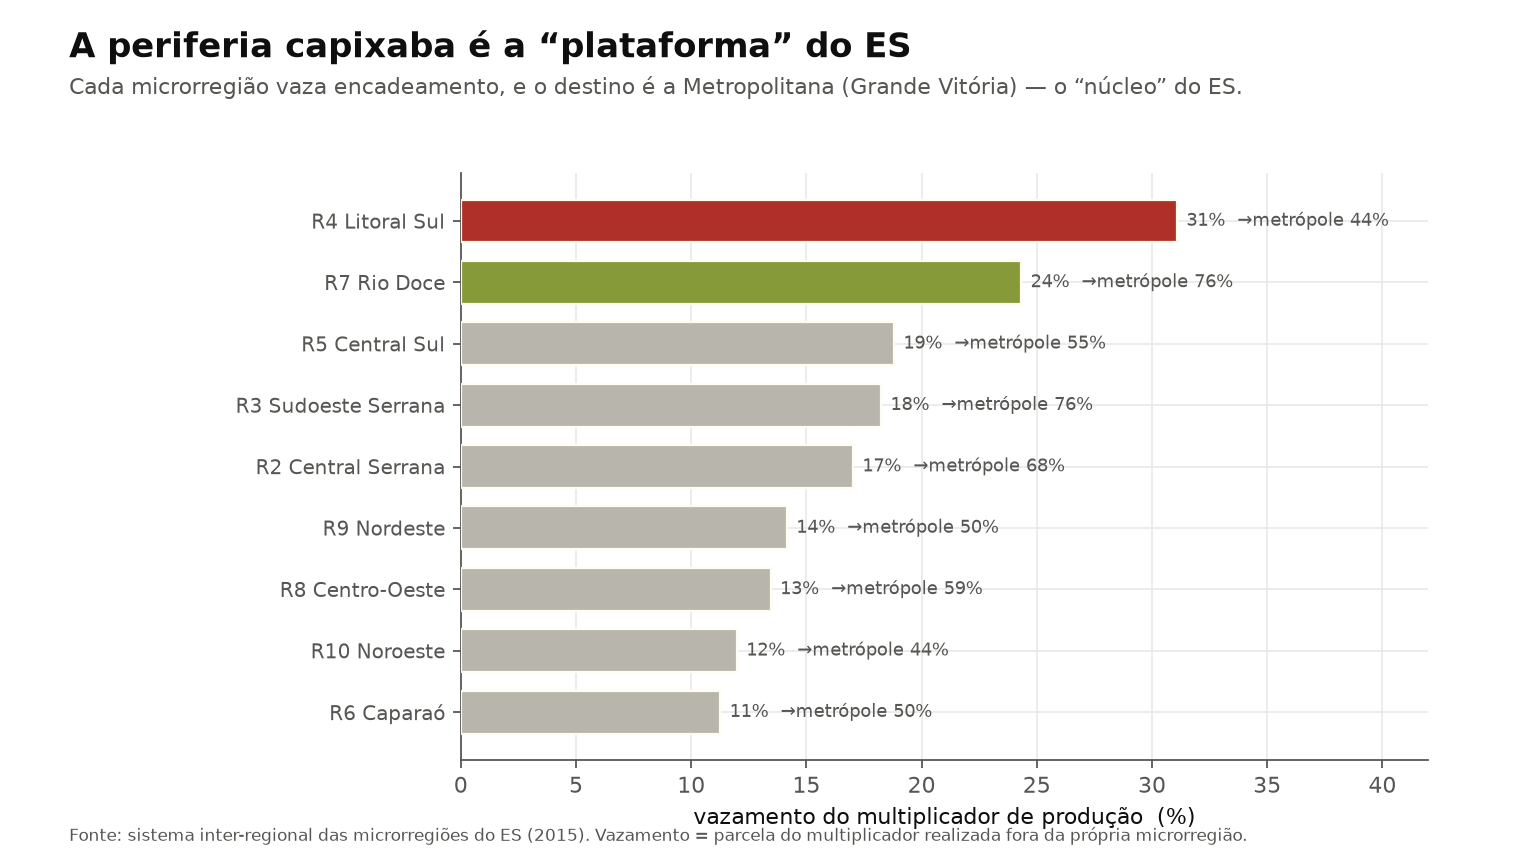
\includegraphics[width=.92\linewidth]{fig_periferia_metropole.png}
\caption{Vazamento do multiplicador de produção por microrregião do ES e parcela
do \emph{spillover} que se destina à Região Metropolitana. A periferia capixaba
exporta encadeamento para o núcleo do estado --- o mesmo papel que o ES exerce
perante o Sudeste.}
\label{fig:periferia}
\end{figure}

A auto-similaridade é mais que qualitativa. O \emph{mesmo} modelo nulo, agora
sobre as 10 microrregiões, devolve a \emph{mesma} regularidade: a razão de
\emph{feedback} cresce com o porte da microrregião, com $R^2=\mathbf{0{,}91}$ ---
ainda mais forte que o 0,59 do nível interestadual (Figura~\ref{fig:fractal}). A
relação que governa estados dentro do Brasil governa microrregiões dentro do ES.
A extração hipotética fecha o argumento: removida a metrópole do sistema, a
produção das demais microrregiões cairia \textbf{13,0\%} --- a periferia depende
do núcleo capixaba como o ES depende do Sudeste.

\begin{figure}[ht]
\centering
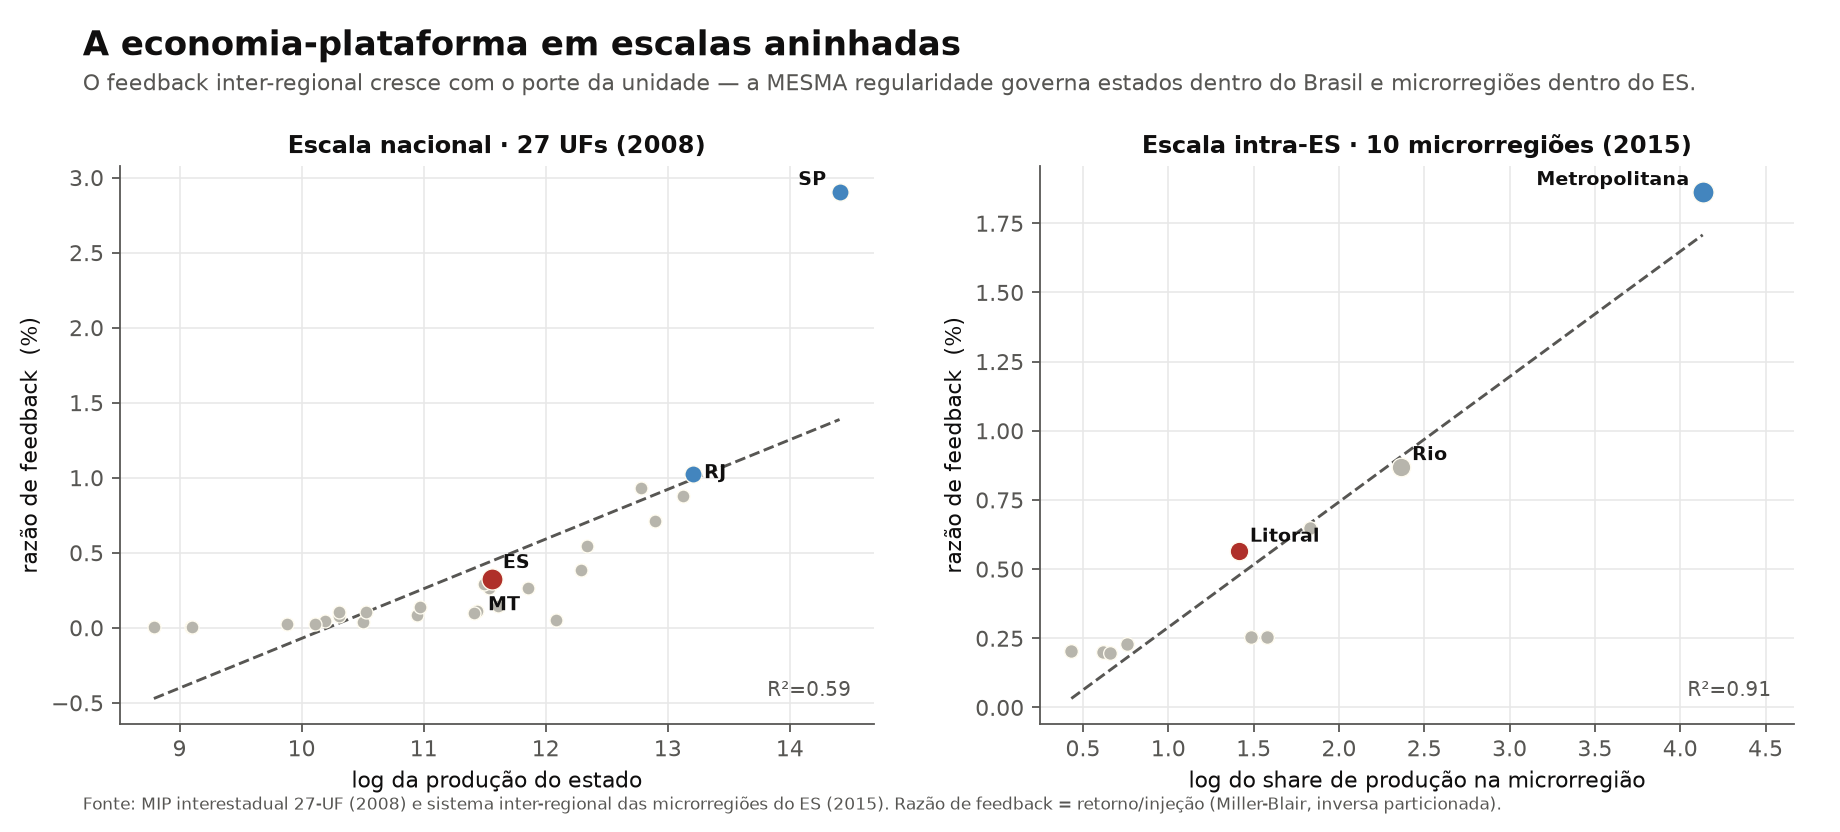
\includegraphics[width=\linewidth]{fractal_duas_escalas.png}
\caption{Invariância de escala. A razão de \emph{feedback} cresce com o porte da
unidade nas duas escalas --- 27 UFs no Brasil (esq., $R^2=0{,}59$) e 10
microrregiões no ES (dir., $R^2=0{,}91$). A mesma mecânica de posição-e-porte
opera em ambas. Fonte: \texttt{16\_fig\_fractal.py}.}
\label{fig:fractal}
\end{figure}

\paragraph{Robustez.} O sistema microrregional apresenta uma coluna desbalanceada
(setor S23, com $\sum_i a_{i,\cdot}=1{,}07$ em todas as 10 regiões); a inversa de
Leontief permanece não-negativa e finita. Excluindo S23 e recomputando, o
vazamento da metrópole passa de 8,4\% a 7,9\% e o $R^2$ do modelo nulo permanece
em 0,91 --- o padrão fractal não é dirigido por esse setor.

% =====================================================================
\section{Discussão}
\label{sec:discussao}
Os dois testes contam uma história única. A \emph{mecânica} da economia-plataforma
--- vazar muito, retornar quase nada, escoar ao núcleo --- não é uma propriedade
do Espírito Santo: é uma regularidade de \emph{posição relativa} e \emph{porte},
que se reproduz \emph{fractalmente} entre escalas. Vale para a microrregião
perante o estado e para o estado perante o país: \emph{periferia} está para o
\emph{ES} assim como o \emph{ES} está para o \emph{Sudeste}. A Grande Vitória é o
``SP/RJ'' do Espírito Santo; o Litoral Sul minerador é o ``ES'' do Espírito
Santo. Reconhecer isso desarma a objeção tautológica de frente: ao mostrar que a
mecânica é genérica \emph{e} invariante de escala, o trabalho deixa de tratá-la
como achado e a recoloca como \emph{pano de fundo} estrutural.

O achado, então, muda de lugar. O que singulariza o ES não é \emph{como} seu
multiplicador se decompõe --- isso o porte prediz ---, mas \emph{de que} ele é
feito: uma pauta mineral/primária, a montante, que o coloca entre os dois estados
de maior intensidade de base do país. A plataforma é uma condição
\emph{composicional}. Essa releitura tem consequência analítica e de política.
Analiticamente, ela explica por que a assimetria \emph{per se} é fraca como
evidência e por que a composição é forte: o vazamento é o \emph{sintoma}; a
pauta primário-exportadora é a \emph{causa}. Para a política, ela desloca o alvo
--- não se trata de ``reduzir o vazamento'' (genérico e, em boa medida,
inescapável para o porte), mas de \emph{adensar} ou \emph{diversificar} a
composição que o gera, e de capturar, via instrumentos fiscais (royalties) ou
ambientais (carbono incorporado), o valor que a composição atual deixa transitar.
A mesma lógica fractal sugere que o problema do ES perante o Sudeste é,
internamente, o problema da periferia capixaba perante a Grande Vitória --- e que
políticas de adensamento precisam de um endereço \emph{sub}-estadual.

% =====================================================================
\section{Limitações}
\label{sec:limites}
\textbf{(i) Fluxos estimados.} Os fluxos inter-regionais e, sobretudo, os
sub-estaduais são \emph{estimados} pelo IIOAS (gravitacional), não observados;
na escala microrregional são ainda mais sintéticos, de modo que o modelo nulo
intra-ES ($n=10$) é indicativo, não inferência. \textbf{(ii) Safras e agregações
heterogêneas.} O benchmark é de 2008 (26 setores) e o sistema microrregional de
2015 (35 setores); a comparação entre escalas é de \emph{lógica}, não um
cruzamento numérico direto. \textbf{(iii) Sem emprego na escala fina.} O sistema
microrregional traz apenas remunerações (não o vetor de pessoal ocupado), de modo
que o vazamento de \emph{emprego} não é replicável intra-ES. \textbf{(iv) Chave
das microrregiões.} A correspondência entre os blocos $R1\!-\!R10$ e os nomes
oficiais segue a ordem da Lei 9.768/2011, corroborada pelo porte e pela geografia
econômica (a Metropolitana é o maior bloco; o Litoral Sul, sede de Anchieta, é o
de maior vazamento); a conferência fina contra os arquivos-fonte de cada
microrregião fica registrada. \textbf{(v) Desbalanço S23}, tratado em
\S\ref{sec:fractal}.

% =====================================================================
\section{Conclusão}
\label{sec:conclusao}
A economia-plataforma é fractal. Sua mecânica --- alto vazamento, \emph{feedback}
quase nulo, encadeamento que escoa ao núcleo --- não é um traço idiossincrático do
Espírito Santo, mas uma regularidade de posição-e-porte que governa, com a mesma
forma, estados dentro do Brasil ($R^2=0{,}59$) e microrregiões dentro do ES
($R^2=0{,}91$). O que é próprio do ES é a sua \emph{composição}: uma pauta
mineral/primária, a montante, que o situa entre os dois estados de maior base do
país. Deslocar a leitura da decomposição para a composição torna a tese ao mesmo
tempo mais honesta --- porque concede o que é genérico --- e mais útil --- porque
aponta a alavanca certa: não o vazamento, mas a pauta que o produz, em cada escala
em que a plataforma se repete.

% =====================================================================
\begin{thebibliography}{99}

\bibitem[Guilhoto \& Sesso Filho(2005)]{guilhoto2005estimacao}
Guilhoto, J. J. M., \& Sesso Filho, U. A. (2005). Estimação da matriz
insumo-produto a partir de dados preliminares das contas nacionais.
\textit{Economia Aplicada}, 9(2), 277--299.

\bibitem[Haddad et al.(2017)]{haddad2017iioas}
Haddad, E. A., Gonçalves Júnior, C. A., \& Nascimento, T. O. (2017).
Matriz interestadual de insumo-produto para o Brasil: uma aplicação do método
IIOAS. \textit{Revista Brasileira de Estudos Regionais e Urbanos}, 11(4),
424--446.

\bibitem[Isard(1951)]{isard1951}
Isard, W. (1951). Interregional and regional input-output analysis: a model
of a space-economy. \textit{The Review of Economics and Statistics}, 33(4),
318--328.

\bibitem[Miller(1966)]{miller1966}
Miller, R. E. (1966). Interregional feedback effects in input-output models: some
preliminary results. \textit{Papers of the Regional Science Association}, 17, 105--125.

\bibitem[Miller \& Blair(2009)]{millerblair2009}
Miller, R. E., \& Blair, P. D. (2009). \textit{Input-Output Analysis:
Foundations and Extensions}. 2nd ed. Cambridge University Press.

\bibitem[Round(1983)]{round1983nonsurvey}
Round, J. I. (1983). Nonsurvey techniques: a critical review of the theory and the
evidence. \textit{International Regional Science Review}, 8(3), 189--212.

\end{thebibliography}

\end{document}
